\subsubsection{30.11.14}

\begin{enumerate}
	\item The time of beginning and ending of the meeting:
	14:00 - 20:00
	\item Purposes of the meeting:
	\begin{enumerate}
		\item To change the gripper for balls.
		
		\item To test the new gripper.
		
	\end{enumerate}
	\item Work that has been done:
	\begin{enumerate}
		\item They were installed plastic blades on the axle.
		
		\begin{figure}[H]
			\begin{minipage}[h]{0.2\linewidth}
				\center  
			\end{minipage}
			\begin{minipage}[h]{0.6\linewidth}
				\center{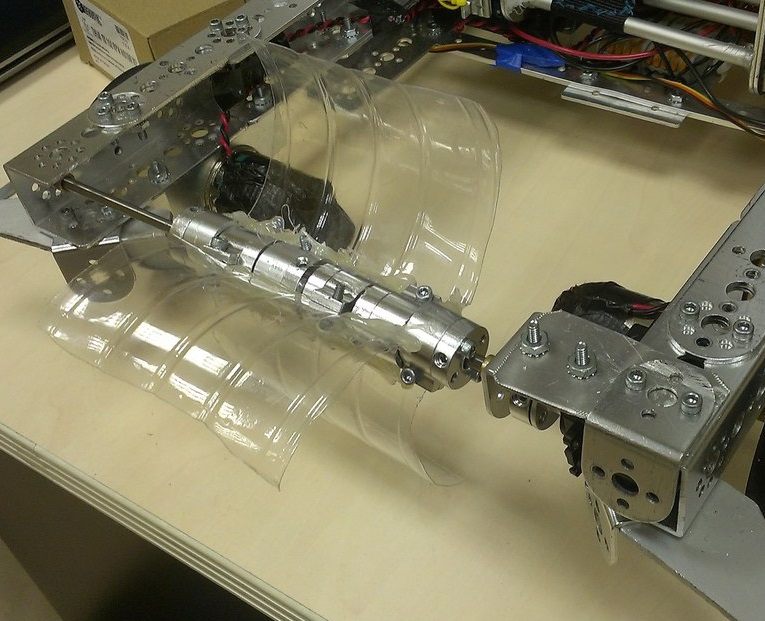
\includegraphics[scale=0.25]{days/30.11.14/images/01}}
				\caption{The new gripper for balls}
			\end{minipage}
		\end{figure}
		
		\item Tests.
		
		\item The transverse beam prevented to working of gripper because blades more stiffness than ties. So the beam was removed. It was decided to install U-shaped rib of rigidity. Horizontal crossbar of it will locate higher and will not prevent to working of the gripper.
		
		\item The axle of gripper was located too low. So it was decided to increase clearance of front wheels. After incrementation of clearance gripper hasn't any problem with capture of big balls.
		
	%	\begin{figure}[H]
	%		\begin{minipage}[h]{0.2\linewidth}
	%			\center  
	%		\end{minipage}
	%		\begin{minipage}[h]{0.6\linewidth}
	%			\center{
\includegraphics[scale=0.3]{days/30.11.14/images/02}}
	%			\caption{Клиренс увеличен}
	%		\end{minipage}
	%	\end{figure}
		
	\end{enumerate}
	
	\item Results: 
	\begin{enumerate}
		\item Gripper for balls was changed.
		
		\item Clearance of front wheels was increased.
		
		\item Gripper was tested.Result positive.
		
		\item Transverse rib of rigidity was removed.
		
	\end{enumerate}
	
	\item Tasks for the next meetings:
	\begin{enumerate}
		\item To move the MOB to top of the last slat.
		
		\item To install П-shaped rib of rigidity.
		
		\item To start elaboration of concept of the new bucket.
		
	\end{enumerate}     
\end{enumerate}
\fillpage